\chapter{Abordagem Proposta} \label{chap:propApproach}
	\begin{myenv}{1.5}
		\section{Coleta de dados}
			\par No tocante a base de dados de comparação a escolha foi de criar uma a partir dos locutores existentes nos arredores da universidade e dentro dela. Os locutores foram escolhidos de acordo com seu sexo e idade de forma que a amostra estudada tenha uma abrangência que cubra desde crianças em época pré-escolar até adultos entre 50 e 60 anos do sexo masculino e feminino. Cada entrevistado ditou os dígitos de 0 a 9 em inglês e português.
			
			\par Um total de 21 indivíduos foram entrevistados, totalizando um total de 20 amostras já que, em um dos casos, não foi possível coletar todos os dados necessários.
			
			\par Cada uma das gravações foram feitas em ambientes distintos com diferentes níveis de ruído de fundo garantindo uma boa variabilidade de interferências que certamente irão impactar nos resultados dos classificadores que serão usados.
			
			\par Coletadas as amostras, os dígitos das mesmas foram separados um-a-um, usando uma ferramenta desenvolvida para esse fim, resultando em uma base de dados com 820 trechos. No apêndice deste documento é possível ter acesso a ferramenta criada para auxiliar na preparação desta base de dados.
			
			\subsection{Base de dados de áudios originais}
				\par Para a constituição da base de dados não regravada os áudios originais foram editados e separados digito a dígito.
	
			\subsection{Base de dados de áudios regravados}
				\par No caso da base usada para simulação de \textit{voice spoofing} foi criado um arquivo contendo todas as falas de todos os entrevistados, em seguida, os sons reproduzidos por este foram regravados por um segundo dispositivo de gravação diferente do original.

			\subsection{Organização}
				\par A organização da base de dados se deu por tipo (regravado ou não), idioma, dígito ditado e interlocutor considerado. Foi criada uma estrutura hierárquica de diretórios de forma a permitir que fosse fácil e intuitivo acessar cada uma das amostras seja por vias automatizadas ou não. Os arquivos regravados residem no diretório "playback" \ já os não regravados se encontram em "live".	Essa organização é mostrada nas figuras \ref{fig:directorystructlevel01}, \ref{fig:directorystructlevel02} e \ref{fig:directorystructlevel03}.
				
				\par Para facilitar a automação do processamento foram criados três arquivos de texto:
				\begin{itemize}
					\item \textit{dataSurvey.txt}: Contêm os dados de idade e sexo de cada entrevistado.
					\item \textit{inputListLive.txt}: Uma lista de caminhos para todos os arquivo não regravados.
					\item \textit{inputListSpoofing.txt}: Apresenta uma listagem dos caminhos para todos os arquivos regravados.
				\end{itemize}
			
				\par Apenas para ilustrar o conteúdo do diretório \textbf{"separated \textfractionsolidus live \textfractionsolidus en\_US \textfractionsolidus 0"} se constitui de vários arquivos do tipo \textit{wave} cada um identificando o locutor ao qual pertence como mostrado na  figura \ref{fig:directorystructlevel03}.

					
				\begin{figure}
					\center
					\subfigure[Base em nível 1]{
						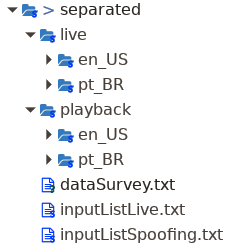
\includegraphics[width=.3333\linewidth]{images/directoryStructLevel01}
						\label{fig:directorystructlevel01}
					}
					\subfigure[Base em nível 2]{
						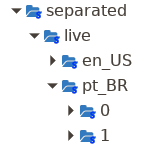
\includegraphics[width=.2\linewidth]{images/directoryStructLevel02}
						\label{fig:directorystructlevel02}
					}
					\subfigure[Base em nível 3]{
						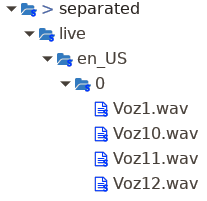
\includegraphics[width=.3333\linewidth]{images/directoryStructLevel03}
						\label{fig:directorystructlevel03}
					}
					\caption{Organização da base de dados}
				\end{figure}
			
			

			
			
			
			
			
		\pagebreak
		\newpage
		\section{Experimentos}
		\par 
		
	\end{myenv}